% 问题三
\section{问题三的模型建立与求解}

\subsection{问题分析}

问题三要求在单品层面给出 7 月 1 日的补货量与定价策略：以 2023 年 6 月 24--30 日的可售品种为候选，可售单品总数控制在 27--33 个，各单品订购量满足最小陈列量 2.5 千克，在“尽量满足市场对各品类蔬菜商品需求”的前提下使商超收益最大。

与问题二（品类级、周计划、报童 + 解析定价）相比，问题三有两个本质变化：
\begin{enumerate}
    \item \textbf{决策粒度下放到单品}：问题二的决策对象是 6 个品类的日补货总量与加价率，问题三的决策对象是每个单品的“是否上架—选哪档价—订多少货”三件事；
    \item \textbf{引入耦合约束}：可售单品总数 27--33 与单品最小陈列量 2.5 kg 是两个跨单品的共享约束，使单品之间不能按问题二“逐品类独立优化”的方式拆解，必须建立\textbf{单品级联合优化}模型 \cite{kok2009,vanryzin1999}。
\end{enumerate}

本题有三个突出难点：
\begin{enumerate}
    \item \textbf{单品弹性不可识别}：单品历史样本短、价格变异少，直接回归得到的单品弹性方差极大，且部分单品价格长期不变、价格档位稀疏，必须借用问题二的品类弹性先验做收缩（Shrinkage）估计 \cite{efron1977,james1961,montgomery1997}；
    \item \textbf{非线性利润 + 离散选品的耦合}：若每个单品同时决策“连续售价 × 连续订购量”，利润目标为多品非线性混合整数规划，难以保证全局最优；将连续售价离散为有限档价格网格后，目标转化为线性 MIP \cite{talluri2004,wolsey1998}；
    \item \textbf{“尽量满足需求”的量化}：题面要求“尽量满足市场对各品类蔬菜商品需求”，本文以单品缺货惩罚（软约束）刻画，并以总体/品类满足率作为可追溯的输出指标，配合惩罚系数灵敏度（详见第九章）给出“满足率—收益”的权衡证据 \cite{khouja1999,petruzzi1999}。
\end{enumerate}

基于上述分析，本问按“\textbf{候选集定义 → 单品需求建模 → 离散价格网格 → MIP 组合优化 → 灵敏度校验}”五步建模：
\begin{itemize}
    \item 第一步，以 2023-06-24~30 实际在售、批发价可得、周均净销量不低于 0.5 kg/天的单品构成候选集 $S$（共 45 个），避免无需求或无批发价的单品进入决策；
    \item 第二步，延续问题二的常弹性（幂律）需求结构，单品弹性用 Shrinkage 向品类弹性收缩，得到单品需求函数 $D_i(p)$（见 2.2 节）；
    \item 第三步，把每个单品的候选售价离散为历史价格区间内的 $K=11$ 档网格，使利润目标线性化（见 3.1 节）；
    \item 第四步，建立 0-1 MIP，同时决策上架单品（27--33 个）、各单品价格档位与订购量，目标为“收入 − 进货成本 − 缺货惩罚”，并施加最小陈列量、定价唯一、可售上限与品类覆盖约束（见 3.2--3.4 节）；
    \item 第五步，用 HiGHS 求解（报告状态与最优性 gap），缺货惩罚、选品数、弹性、批发价、损耗率、价格网格与大 M 的灵敏度分析统一在第九章报告 \cite{huangfu2018}。
\end{itemize}
模型结论直接回答题面：7 月 1 日上架 33 个单品（各品类均覆盖），给出每个单品的售价、订购量与预期收益，需求满足率 1.00、总利润 682.08 元。

\subsection{模型准备}

\subsubsection{数据来源与整合}

本问使用附件 1--4：单品—品类映射与单品名称来自附件 1；单品日净销量 $Q_{i,t}$ 与日售价 $p_{i,t}$ 由附件 2 按单品聚合（退货以负销量并入当日净销量）；单品批发价 $W_i$ 来自附件 3（按单品 ffill，仍缺失者用单品历史均值补齐）；损耗率 $L_i$ 取自附件 4 单品损耗率（百分数，代入公式前除以 100），分类级损耗率用于交叉校验。以上口径与第 1、2 题完全一致，不重复清洗。

\subsubsection{单品级需求模型：幂律需求与 Shrinkage 弹性}

\textbf{模型设定}。延续问题二的常弹性（幂律）需求结构 \cite{tellis1988,hoch1995}，单品 $i$ 在售价 $p$ 下的日需求为
\begin{equation}
D_i(p)=d_i\left(\frac{p}{p_i^0}\right)^{\hat\beta_i},
\end{equation}
其中 $d_i$ 为参考价下的基准日需求（kg/日），$p_i^0$ 为参考价（元/kg），$\hat\beta_i$ 为 Shrinkage 修正后的单品价格弹性（预期为负）。该式把问题二的品类弹性结构下放到单品，保证两问的需求函数口径一致。

\textbf{单品弹性估计与 Shrinkage 收缩}。对价格有变异的单品独立回归：
\begin{equation}
\ln Q_{i,t}=\alpha_i+\beta_{\mathrm{raw},i}\ln p_{i,t}+\delta_i\,t+\sum_{k=1}^{6}\delta_{i,k}\mathbb{1}_{\{\mathrm{weekday}=k\}}+\sum_{m=1}^{11}\eta_{i,m}\mathbb{1}_{\{\mathrm{month}=m\}}+\varepsilon_{i,t},
\end{equation}
其中 $\beta_{\mathrm{raw},i}$ 为原始弹性。采用经验贝叶斯收缩 \cite{efron1977,james1961,montgomery1997}：
\begin{equation}
\hat\beta_i = w_i\beta_{\mathrm{raw},i}+(1-w_i)\beta_{c(i)},\qquad w_i=\frac{N_i}{N_i+M_0},
\end{equation}
其中 $N_i$ 为有效回归样本量（价格发生变动的观测天数），$M_0=30$ 为先验权重常数。

\textbf{弹性兜底}：若 $N_i<N_{\min}=14$ 或价格无变异，令 $\hat\beta_i=\beta_{c(i)}$；若收缩后 $\hat\beta_i>0$，同样令 $\hat\beta_i=\beta_{c(i)}$。不设人工弹性下界，弱弹性单品最优价落在网格上界属正常边界解，与问题二口径一致。实测 45 个候选中 12 个借用品类弹性；选中 33 个单品中 10 个借用品类弹性，收缩弹性区间为 $[-2.52,-0.03]$，均值 -0.44。

\subsubsection{基准需求与参考价口径}
\begin{itemize}
    \item $d_i$：6/24--30 日均净销量；销售天数不足 3 天的单品用近 4 周日均可替代，并标注“低样本”；
    \item $p_i^0$：6/24--30 销量加权均价；
    \item $W_i$：6/24--30 批发价均值；
    \item 价格百分位区间 $[P_5,P_{95}]$ 以近 4 周（2023-06-03~06-30）为基准。
\end{itemize}

\subsubsection{符号说明}

\begin{table}[htbp]
\centering
\caption{问题三符号说明}
\label{tab:q3_symbols}
\begin{tabular}{l l l}
\toprule
符号 & 含义 & 单位 \\
\midrule
$S$ & 候选单品集 & --- \\
$y_i\in\{0,1\}$ & 单品 $i$ 是否上架 & --- \\
$p_{i,k}$ & 单品 $i$ 第 $k$ 档候选价（$K=11$ 档） & 元/kg \\
$x_{i,k}\in\{0,1\}$ & 单品 $i$ 是否选择第 $k$ 档价格 & --- \\
$q_i\ge 0$ & 单品 $i$ 订购量 & kg \\
$s_i\ge 0$ & 单品 $i$ 实际销量 & kg \\
$u_i\ge 0$ & 单品 $i$ 缺货量 & kg \\
$z_{i,k}\ge 0$ & 第 $k$ 档价格下的实际销量（线性化辅助变量） & kg \\
$D_{i,k}$ & 第 $k$ 档价格下的需求点估计 & kg \\
$d_i,\ p_i^0$ & 基准日需求、参考价 & kg，元/kg \\
$\hat\beta_i,\ \beta_{c(i)}$ & 单品弹性、品类弹性 & --- \\
$W_i$ & 单品批发价 & 元/kg \\
$L_i$ & 单品损耗率 & --- \\
$\gamma_i$ & 单品缺货惩罚 & 元/kg \\
$\rho$ & 缺货惩罚调节系数（基准 1.0） & --- \\
$M_i$ & 单品订购量上界（大 M） & kg \\
$K$ & 价格档位数（基准 11） & --- \\
$\mathcal{C}_c$ & 品类 $c$ 的单品集合 & --- \\
$\mathrm{FR},\ \mathrm{FR}_c$ & 总体/品类需求满足率 & --- \\
\bottomrule
\end{tabular}
\end{table}

\subsection{模型建立}

\subsubsection{离散价格网格}

把每个单品的价格区间取历史售价百分位区间 $[\min(P_5,p_i^0),\max(P_{95},p_i^0)]$，离散为 $K=11$ 档候选价 $p_{i,k}$（$k=1,\dots,K$），并把参考价 $p_i^0$ 显式并入网格（去重后取 $K$ 档）。网格生成规则默认等距，灵敏度分析（详见第九章）对比 $K=7$ 与分位数取点两种口径。若 $|\hat\beta_i|>1$，内点最优价 $p_i^*=\dfrac{E_i}{E_i-1}\cdot\dfrac{W_i}{1-L_i}$（$E_i=|\hat\beta_i|$）可作为网格内插参考。

\subsubsection{目标函数}

\begin{equation}
\max\quad \sum_{i\in S}\left(\sum_{k=1}^{K}p_{i,k}\,z_{i,k}-W_i\,q_i-\gamma_i\,u_i\right).
\end{equation}
其中第一项为销售收入，第二项为进货成本（口径统一为“$q_i$ = 订购量”），第三项为缺货惩罚。单位缺货惩罚取机会损失毛利并截尾：
\begin{equation}
\gamma_i=\rho\cdot\max\left(0,\ p_i^0-\frac{W_i}{1-L_i}\right),\qquad \rho\in\{0.5,1.0,1.5\},
\end{equation}
$\rho$ 基准取 1.0，灵敏度分析见第九章。

\subsubsection{约束条件}

(1) \textbf{选品数约束}：
\begin{equation}
27\le \sum_{i\in S}y_i\le 33;
\end{equation}

(2) \textbf{订购量上下限（最小陈列量）}：
\begin{equation}
2.5\,y_i\le q_i\le M_i\,y_i,\qquad \forall i\in S;
\end{equation}

(3) \textbf{定价唯一性}：
\begin{equation}
\sum_{k=1}^{K}x_{i,k}=y_i,\qquad \forall i\in S;
\end{equation}

(4) \textbf{销量与线性化}：
\begin{equation}
s_i=\sum_{k=1}^{K}z_{i,k},\qquad s_i\le q_i(1-L_i),\qquad z_{i,k}\le D_{i,k}\,x_{i,k},\qquad z_{i,k}\ge 0;
\end{equation}

(5) \textbf{缺货量}：
\begin{equation}
u_i=\sum_{k=1}^{K}D_{i,k}\,x_{i,k}-s_i,\qquad \forall i\in S;
\end{equation}

(6) \textbf{品类覆盖}：
\begin{equation}
\sum_{i\in\mathcal{C}_c}y_i\ge 1,\qquad \forall c;
\end{equation}
需求满足率输出指标为
\begin{equation}
\mathrm{FR}=\frac{\sum_i s_i}{\sum_i\sum_k D_{i,k}x_{i,k}},\qquad \mathrm{FR}_c=\frac{\sum_{i\in\mathcal{C}_c}s_i}{\sum_{i\in\mathcal{C}_c}\sum_k D_{i,k}x_{i,k}}.
\end{equation}

\subsubsection{大 M 取值与求解算法}

订购量上界取
\begin{equation}
M_i=\max\left(3\cdot\max_{t}Q_{i,t}^{\mathrm{hist}},\ 2.5,\ 1.05\,D_{i,1}\right),
\end{equation}
其中 $D_{i,1}$ 为最低档价格下的需求。用 HiGHS（\texttt{scipy.optimize.milp}）求解 0-1 MILP \cite{huangfu2018}，时间上限 60 秒，报告求解状态、最优性 gap 与节点数。基准 case 求解状态为 optimal（status=0）、gap=0、节点数 1、无降级。

\subsubsection{与问题一、问题二的衔接}

\begin{itemize}
    \item \textbf{弹性承接}：品类弹性取自问题二 Log-Log 回归，需求函数同为常弹性幂律形式；
    \item \textbf{分布衔接（问题一）}：问题一给出品类日销量分布，问题三为确定性单日优化，分布仅在随机化改进中进入；
    \item \textbf{选品衔接（问题一）}：问题一协同变动网络与聚类为问题三提供候选分组框架 \cite{kok2009}；
    \item \textbf{补货量交叉核对}：$\sum_{i\in\mathcal{C}_c}q_i(1-L_i)$ 与问题二 7 月 1 日期望需求 $\mu_{c,t}(P^*)$ 比值 0.21~0.74，差异为口径差异（详见第九章）。
\end{itemize}

\subsection{模型求解与结果分析}

\subsubsection{候选集与单品弹性估计结果}

候选集构成与品类弹性见表 3。

\begin{table}[htbp]
\centering
\caption{候选集构成与品类弹性}
\label{tab:q3_candidates}
\begin{tabular}{l r r r}
\toprule
品类 & 候选单品数 & 品类弹性 $\beta_c$ & 弹性绝对值 $\lvert\beta_c\rvert$ \\
\midrule
花叶类 & 16 & -0.45 & 0.45 \\
花菜类 & 2 & -0.50 & 0.50 \\
水生根茎类 & 6 & -0.07 & 0.07 \\
茄类 & 4 & -0.26 & 0.26 \\
辣椒类 & 9 & -0.13 & 0.13 \\
食用菌 & 8 & -0.31 & 0.31 \\
合计 & 45 & --- & --- \\
\bottomrule
\end{tabular}
\end{table}

单品弹性诊断：45 个候选的有效样本量 $N_i$ 为 28~559；13 个单品原始弹性为正，其中 12 个借用品类弹性；选中单品收缩弹性区间 $[-2.52,-0.03]$，均值 -0.44。

\subsubsection{组合优化求解与决策结果}

MIP 一次求解即达最优，约束校验全部通过。总体结果见表 4。

\begin{table}[htbp]
\centering
\caption{问题三总体求解结果}
\label{tab:q3_overall}
\begin{tabular}{l r}
\toprule
指标 & 数值 \\
\midrule
候选单品数 & 45 \\
选中单品数 & 33 \\
总订购量 & 296.83 kg \\
损耗后可售量 & 271.19 kg \\
总销量 / 总需求 & 270.14 kg / 270.14 kg \\
总缺货量 & 0.00 kg \\
总收入 & 1915.69 元 \\
进货总成本 & 1233.61 元 \\
缺货惩罚 & 0.00 元 \\
总利润 & 682.08 元 \\
需求满足率 FR & 1.00 \\
陈列刚性超订量 & 1.16 kg（10.53 元） \\
\bottomrule
\end{tabular}
\end{table}

单品毛利 Top 10 见表 5，完整决策表见附录 A1。

\begin{table}[htbp]
\centering
\caption{2023-07-01 主要单品决策摘要（按单品毛利排序，Top 10）}
\label{tab:q3_top10}
\begin{tabular}{r l l r r r r}
\toprule
序号 & 单品名称 & 品类 & 售价（元/kg） & 订购量（kg） & 预计销量（kg） & 单品毛利（元） \\
\midrule
1 & 小米椒(份) & 辣椒类 & 7.66 & 22.82 & 20.67 & 109.49 \\
2 & 西兰花 & 花菜类 & 14.83 & 12.06 & 10.95 & 67.93 \\
3 & 竹叶菜 & 花叶类 & 7.54 & 10.01 & 8.65 & 42.00 \\
4 & 紫茄子(2) & 茄类 & 6.89 & 11.09 & 10.42 & 30.23 \\
5 & 西峡花菇(1) & 食用菌 & 24.00 & 5.18 & 4.62 & 30.11 \\
6 & 金针菇(盒) & 食用菌 & 3.55 & 13.29 & 13.23 & 27.64 \\
7 & 木耳菜 & 花叶类 & 7.71 & 6.24 & 5.77 & 24.43 \\
8 & 云南油麦菜(份) & 花叶类 & 4.29 & 23.36 & 21.15 & 23.94 \\
9 & 长线茄 & 茄类 & 14.00 & 3.91 & 3.64 & 23.68 \\
10 & 芜湖青椒(1) & 辣椒类 & 5.20 & 15.09 & 14.23 & 22.93 \\
\bottomrule
\end{tabular}
\end{table}

\subsubsection{品类结构与收益解读}

图 1 给出候选与选中单品分品类构成。

\begin{figure}[htbp]
\centering
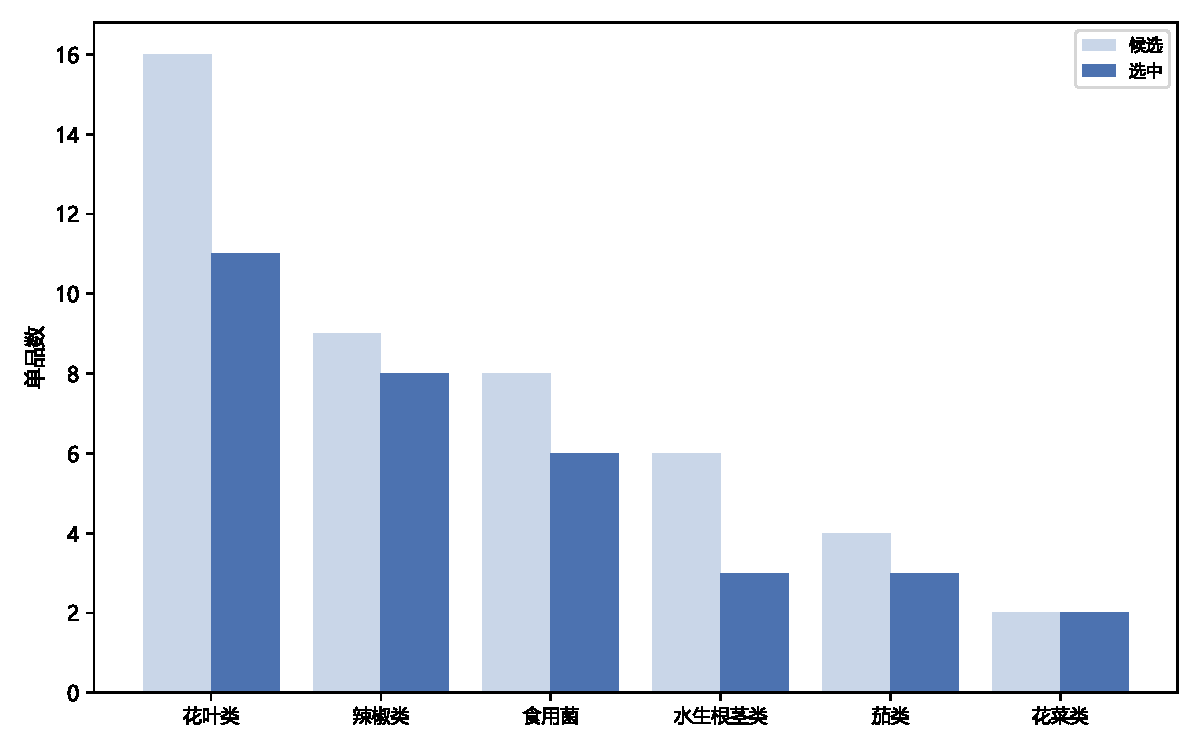
\includegraphics[width=0.8\linewidth]{figures/q3_selection.pdf}
\caption{候选与选中单品的分品类构成（柱状图，浅色为候选、深色为选中）}
\label{fig:q3_selection}
\end{figure}

分品类汇总见表 6。

\begin{table}[htbp]
\centering
\caption{分品类决策汇总}
\label{tab:q3_by_category}
\begin{tabular}{l r r r r r r r}
\toprule
品类 & 选中数 & 订购量合计（kg） & 可售量合计（kg） & 销量（kg） & 需求（kg） & 毛利合计（元） & 毛利占比 \\
\midrule
花叶类 & 11 & 124.03 & 111.20 & 111.20 & 111.20 & 201.99 & 29.6\% \\
辣椒类 & 8 & 81.35 & 74.18 & 73.76 & 73.76 & 220.56 & 32.3\% \\
食用菌 & 6 & 43.89 & 42.60 & 42.60 & 42.60 & 91.30 & 13.4\% \\
花菜类 & 2 & 15.90 & 14.42 & 14.42 & 14.42 & 80.11 & 11.7\% \\
茄类 & 3 & 17.82 & 16.74 & 16.74 & 16.74 & 58.56 & 8.6\% \\
水生根茎类 & 3 & 13.85 & 12.06 & 11.43 & 11.43 & 29.55 & 4.3\% \\
合计 & 33 & 296.83 & 271.19 & 270.14 & 270.14 & 682.08 & 100.0\% \\
\bottomrule
\end{tabular}
\end{table}

主要结果解读：
\begin{itemize}
    \item \textbf{选品结构}：最优解取到选品数上界 33 个，6 个品类全部覆盖；
    \item \textbf{满足率}：总体与各品类满足率均为 1.00；
    \item \textbf{利润来源}：辣椒类（220.56 元）与花叶类（201.99 元）合计占 62%，小米椒(份) 单品毛利 109.49 元；
    \item \textbf{定价行为}：弱弹性单品售价落在网格上界附近，弹性充分单品（西峡花菇 -2.52）取参考档 24.00 元/kg。
\end{itemize}

图 2 展示售价—订购量散点。

\begin{figure}[htbp]
\centering
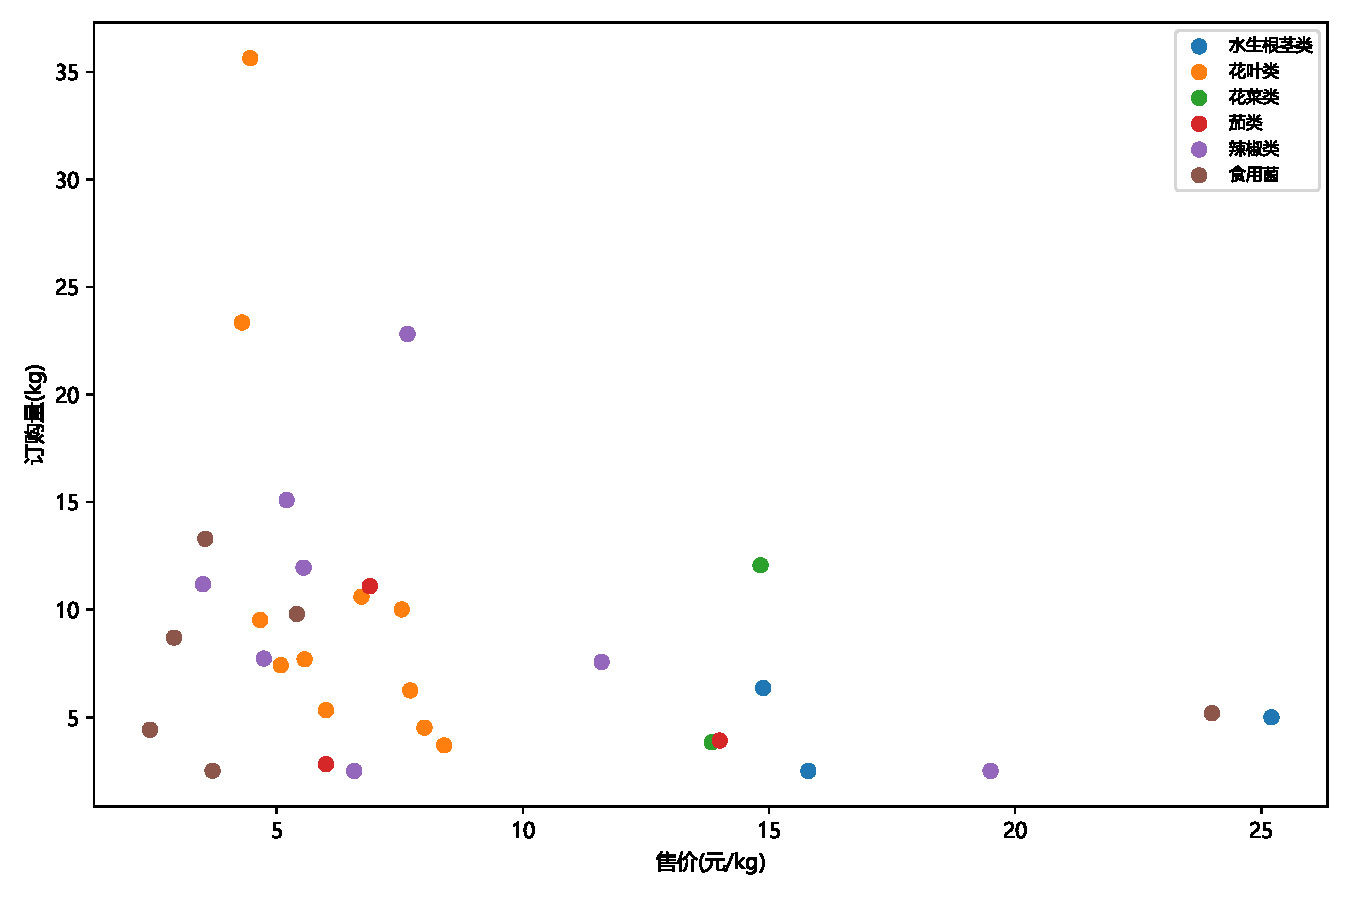
\includegraphics[width=0.8\linewidth]{figures/q3_price_qty.pdf}
\caption{选中单品售价—订购量散点（按品类着色）}
\label{fig:q3_price_qty}
\end{figure}

\subsubsection{决策时序与操作含义}

策略执行分三步：① 确定候选集与弹性、生成网格；② 求解 MIP 得到上架清单、售价档位与订购量；③ 当日执行。定价基于 6/24--30 批发价锁定，若实际批发价偏离，毛利变化见第九章灵敏度分析。

\subsubsection{小结}

问题三建立了单品级选品、定价与补货联合优化框架。以 45 个候选单品，在选品数 27--33、最小陈列量 2.5 kg 约束下，最优方案上架 33 个单品，总利润 682.08 元，满足率 1.00。灵敏度分析详见第九章，结论稳健；与问题二交叉核对通过。操作层面应优先保障小米椒(份)、西兰花等高毛利单品备货。

\textbf{局限与展望}：
\begin{itemize}
    \item 单品需求独立假设，无替代效应 \cite{kok2007,vanryzin1999}；
    \item 确定性需求未考虑随机性，可升级为单品级报童 \cite{federgruen1999,petruzzi1999}；
    \item 净销量低估真实需求 \cite{agrawal1996}；
    \item 未按周末偏置上调基准需求，结果偏保守；
    \item 满足率为软惩罚，可改为硬约束或鲁棒选品 \cite{vanryzin1999,rusmevichientong2012}；
    \item 未考虑动态折扣 \cite{elmaghraby2003} 与品类角色差异 \cite{dhar2001}。
\end{itemize}